\documentclass{article}
\usepackage{graphicx}
\usepackage[margin=1.5cm]{geometry}
\usepackage{amsmath}

\begin{document}
\twocolumn

\title{Monday warm-up: Kinematics, II}
\author{Prof. Jordan C. Hanson}

\maketitle

\section{Memory Bank}

\begin{enumerate}
\item $v = \frac{\Delta x}{\Delta t}$ ... Average velocity.
\item $v = \frac{dx}{dt}$ ... Instantaneous velocity.
\item $a = \frac{\Delta v}{\Delta t}$ ... Average acceleration.
\item $a = \frac{dv}{dt}$ ... Average acceleration.
\item $x(t) = \frac{1}{2}at^2 + v_i t + x_i$ ... Position versus time, given constant acceleration
\item $v(t) = at + v_i$ ... Speed versus time, given constant acceleration
\end{enumerate}

\section{Chapter 2 - Kinematics, II}

\begin{enumerate}
\item Consider the motion of the system depicted in Fig. \ref{fig:1} (top).  Which of the following is true?
\begin{itemize}
\item A: The speed is negative, then positive, then negative again
\item B: The speed is positive, then negative, then positive again
\item C: The speed is positive, then negative
\item D: Cannot determine from Fig. \ref{fig:1} (top).
\end{itemize}
\item Consider the motion depicted in Fig. \ref{fig:1} (top).  Which of the following is true?
\begin{itemize}
\item A: The acceleration is positive, then negative
\item B: The acceleration is negative
\item C: The acceleration is positive
\item D: The acceleration is negative, then positive
\end{itemize}
\item Suppose a cyclist has a velocity of $15$ m s$^{-1}$ at $t=0$.  If the acceleration is 3 m s$^{-2}$, (a) what is the velocity at $t = 4$ seconds? (b) What is the displacement of the cyclist at $t = 4$ seconds? (c) Is the average velocity different from the instantaneous velocity at $t=0$ or $t=4$ seconds?  \\ \vspace{3cm}
\item Consider the motion of the sytem depicted in Fig. \ref{fig:1} (bottom).  (a) From the given data, calculate the speed of the system at points P and Q. (b) Is the acceleration of the sytem positive or negative?  Estimate the acceleration.
\end{enumerate}

\begin{figure}
\centering
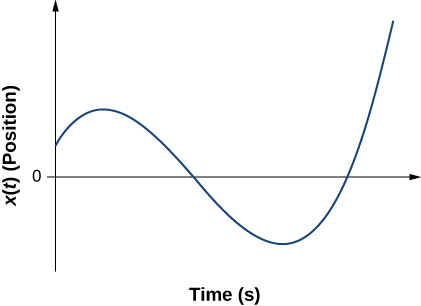
\includegraphics[width=0.4\textwidth]{figures/x_vs_t.jpeg} \hspace{1cm}
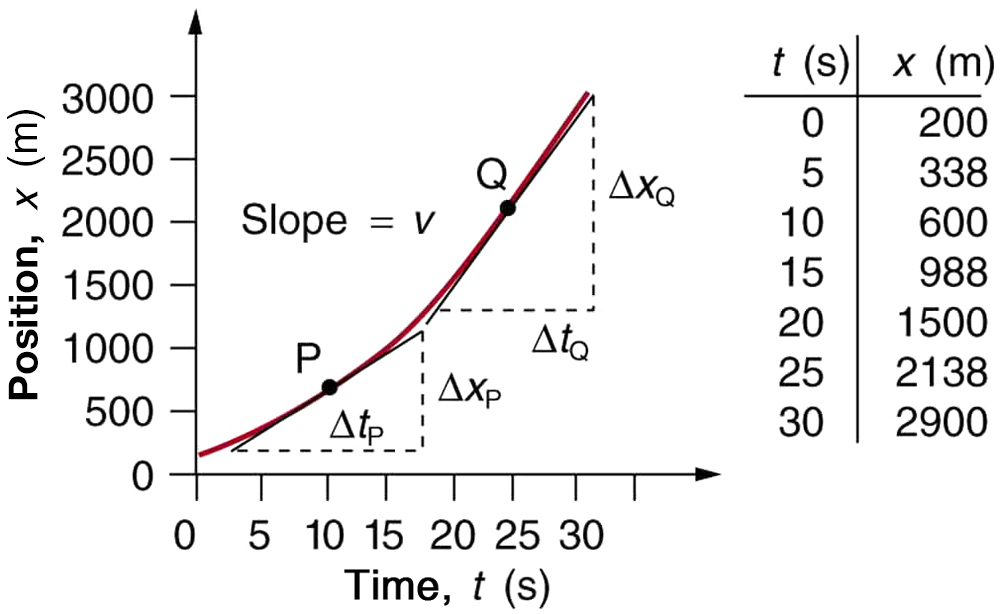
\includegraphics[width=0.4\textwidth]{figures/slope2.jpeg}
\caption{\label{fig:1} (Left) A system moves with constant velocity.  Velocity is the slope on this plot. (Right) A system moves with non-constant velocity.}
\end{figure}


\end{document}
